\documentclass[11pt,a4paper]{article}
\usepackage[margin=25mm]{geometry}
\usepackage[T1]{fontenc}
\usepackage{lmodern,microtype,amsmath,amssymb,amsthm,mathtools}
\usepackage{booktabs,longtable,tabularx,array,enumitem,xcolor,tikz}
\usetikzlibrary{arrows.meta,positioning,fit}
\usepackage[numbers,sort&compress]{natbib}
\usepackage{hyperref}
\hypersetup{colorlinks=true,linkcolor=teal,citecolor=teal,urlcolor=teal,pdftitle={FREM: Causal Fourier-Reservoir Engram Memory for Financial Forecasting}}
\setlist{nosep,leftmargin=*}
\setlength{\parskip}{5pt}
\setlength{\parindent}{0pt}
\setlength{\emergencystretch}{2em}
\newcommand{\R}{\mathbb R}
\newcommand{\E}{\mathbb E}
\newcommand{\F}{\mathcal F}
\newcommand{\M}{\mathcal M}
\newcommand{\ind}{\mathbf 1}
\newcommand{\sg}{\operatorname{stopgrad}}
\newcommand{\softplus}{\operatorname{softplus}}
\newcommand{\clip}{\operatorname{clip}}
\newcommand{\diag}{\operatorname{diag}}
\newtheorem{proposition}{Proposition}
\title{FREM: Causal Fourier--Reservoir Engram Memory for Financial Forecasting and Liability-Aware Allocation}
\author{Research specification prepared for Ryan Gomez}
\date{10 October 2026\\Version 0.1: methods and prospective evaluation manuscript}
\begin{document}
\maketitle
\begin{center}
\fcolorbox{teal}{teal!5}{\parbox{0.92\linewidth}{\textbf{Evidence status: not evaluated.} This release contains an implementation, mathematical specification, research protocol, and handoff. No market-data acquisition, model training, inference, simulation, backtest, or runtime test was executed during authoring. No performance, efficiency, profitability, or empirical novelty claim is established. The manuscript is suitable for methodological review and subsequent experiments; it is not a completed empirical paper.}}
\end{center}

\begin{abstract}
Financial predictors must separate recurring information from transient noise while respecting information availability, execution timing, and investor liabilities. We specify FREM, a candidate architecture combining a temporal joint-embedding predictive objective, a contraction-bounded fixed reservoir, trailing Fourier descriptors, and bounded episodic residual memory. The proposed mechanism is delayed utility credit: an episode influences retention only after its outcome becomes observable, and memories are retained according to realized predictive contribution, spectral surprise, reuse, and age. A feedback controller adjusts a limited set of learning and expert-weighting choices. A separate constrained allocation layer consumes explicitly defined simple-return forecasts or scenarios and protects investor cash-flow obligations. We formalize information timing, the model, fitting, frozen and adaptive inference, uncertainty, cost accounting, and a liability case based on Laura Gao's supplied preparation document. Elementary results establish a reservoir contraction bound, causal forecast measurability under stated assumptions, and a finite-memory bound; they do not establish market predictability. The prospective evaluation compares memory against mechanism-off, alternative-retention, and classical and neural controls using chronological purging, an untouched tail, complete seed families, and date-block inference. Results remain unobserved, and valid negative outcomes are retained as terminal conclusions for this version.
\end{abstract}
\newpage
\begingroup
\small
\setlength{\parskip}{0pt}
\tableofcontents
\endgroup
\newpage

\section{Research question and scope}

The proposed scientific question is narrow: \emph{after controlling information, preprocessing, forecast horizon, and declared training resources, does delayed utility-weighted spectral memory improve out-of-time predictive log score over the same JEPA--reservoir predictor without memory?} A secondary question asks whether any predictive gain survives execution delays, costs, concentration limits, and liability requirements. These are separate claims: improved likelihood does not imply improved trading returns, and improved historical returns do not establish future funding reliability.

The motivating mechanism is that a stable latent encoder can summarize common dynamics while an episodic store preserves unusual but recurring local contexts. Fourier descriptors characterize a trailing window's distribution across frequencies. A reservoir supplies a fixed nonlinear summary of its ordered history. The episodic store retains outcomes and prediction residuals associated with those descriptors. Merely being unusual is insufficient: delayed predictive utility also affects retention. This suggests a discriminating comparison against an equally bounded first-in-first-out store and uniform eviction.

The proposed practical advantage is supported only if the confidence interval clears the prespecified likelihood improvement threshold. An interval at or below zero supports a negative conclusion for the direction of improvement; an interval spanning the practical threshold can remain inconclusive. An advantage that disappears against simpler retention rules weakens the proposed retention mechanism. A methodological defect invalidates the test rather than falsifying the scientific hypothesis. A successful return forecast with noninformative memory would not support the proposed memory mechanism. A sufficiently precise negative result would still determine that this version's extra mechanism is unnecessary in the tested regimes.

The package provides executable research components rather than an assurance that arbitrary data can be made meaningful. Its main forecasting interface requires finite, positive total wealth observations, causal availability metadata, and an explicit executable-observation convention. It supports mapped tabular time-series panels and optional vintage macro features. Images, raw documents, broker order books, missing legal permissions, and zero-recovery defaults are not silently converted into equivalent inputs. A default or delisting with zero terminal recovery needs a separate point-mass outcome model; excluding it to make a backtest pass would invalidate the study.

\section{Prior art and the novelty boundary}

I-JEPA learns representations by predicting target embeddings from context embeddings; its original setting is visual representation learning \citep{assran2023}. Temporal JEPA architectures already exist, including TS-JEPA \citep{ennadir2025}. More recent work reports that the benefit of a particular JEPA instantiation can differ substantially across forecasting backbones \citep{feng2026}. These sources motivate a JEPA-off control and prevent treating the auxiliary objective as inherently beneficial.

Echo-state networks use fixed recurrent dynamics and trained readouts, with stability conditions that must be distinguished from empirical reservoir heuristics \citep{jaeger2001}. Combining reservoir methods and Fourier representations is also established territory: multi-scale random Fourier reservoirs and frequency-domain reservoir computing are close conceptual neighbors \citep{laha2025,fresco2026}. FREM's dense time-domain reservoir plus a trailing DFT is not the frequency-domain recurrence in FRESCO, and no efficiency result from that work transfers automatically.

Engram introduces n-gram-based conditional lookup for language models \citep{cheng2026}. FREM uses the more modest concept of quantized short temporal motifs and an explicit episodic store; it does not reproduce Engram's large static embedding architecture or its constant-time lookup claim. FREM's exact memory search scans its bounded record set and then sorts candidates. Its retrieval cost is therefore explicit rather than assumed negligible.

VICReg motivates variance and covariance penalties against representation collapse \citep{bardes2021}. FREM uses related penalties on context embeddings together with an EMA target, and must measure collapse directly. The feedback controller is a bounded learning-rate, auxiliary-weight, and expert-weight policy. It does not learn a new differentiation operator. Continual backpropagation, which replaces underused units, is a distinct existing idea \citep{dohare2023}; it is not claimed as implemented by the present controller.

XGBoost is gradient tree boosting \citep{chen2016}. It serves as a standalone benchmark and an optional residual corrector. It neither traverses a financial graph nor makes the reservoir run faster. DLinear motivates a simple decomposition-based linear sequence control, while patch-based Transformers motivate a compact tokenized sequence control \citep{zeng2022,nie2022}. The package's task-specific DLinear and patch-Transformer implementations are architectural controls, not claimed reproductions of published state-of-the-art scores.

Repeatedly choosing a strategy because it looks good on the same historical outcomes can overfit the backtest \citep{bailey2015}. Consequently, the package separates development from protected confirmation, retains failed runs, and does not treat a new seed as a new market history. The literature review defines important neighbors but does not establish exhaustive novelty. Before submission, a fuller comparison against directly related retrieval-based financial forecasting systems is necessary.

\begin{table}[ht]
\centering\small
\begin{tabularx}{\linewidth}{p{.23\linewidth}XX}
\toprule Component & Established idea & Candidate contribution to test \\
\midrule JEPA & Predict future latent representations & Whether that objective helps this specific predictor \\
Reservoir and Fourier & Fixed recurrence and frequency features & Whether their stable descriptors improve episode selection \\
Engram memory & Local-pattern lookup and episodic retrieval & Delayed predictive utility governing bounded retention \\
Adaptive controller & Feedback and expert weighting & Whether the declared bounded updates improve stability \\
Stochastic allocation & Scenario risk and constrained optimization & Whether forecasts help after all funding and trading constraints \\
\bottomrule
\end{tabularx}
\caption{The research contribution is not the mere coexistence of seven familiar components.}
\end{table}

\section{Information, observations, and targets}

Let $i\in\{1,\ldots,A\}$ denote an instrument and $t$ a UTC decision timestamp. The available information $\F_t$ contains only observations published by $t$, the instrument master and eligibility known at $t$, and previous matured outcomes. Event time and availability time are separate: a monthly observation stamped January is not available at January's start merely because it describes that month. Revised macro observations require their vintage publication times.

The input $X_{i,t}\in\R^{L\times D}$ is the trailing observed context, accompanied by an ordered feature schema and missingness channels. The future training target context $X^+_{i,t}\in\R^{H\times D}$ is accessed only inside fitting. The public inference call receives $X_{i,t}$ and never uses $X^+_{i,t}$ or its associated future return to construct the current forecast.

The implemented default is next-executable-close research accounting. Let $e_{i,t}$ be the first tradable observation with event time strictly after the decision and let $q_{i,t}$ be the observation $H$ executable intervals later. This conservatively prevents using the close that created the signal as a free simultaneous entry. It does not guarantee an actual fill at the next close. A different entry convention requires a separately specified dataset and protocol version.

With $V_i$ the appropriately reconstructed total-wealth series in base currency,
\begin{equation}
Y_{i,t}=\log\frac{V_i(q_{i,t})}{V_i(e_{i,t})},\qquad
u_{i,t}\ge q_{i,t},
\end{equation}
where $u_{i,t}$ is the outcome-availability timestamp, including the relevant price, distribution, corporate-action, and FX availability. Market returns, forecast locations, and predictive scales use this same horizon. The separate allocation layer requires \emph{simple} returns, not these log-return locations.

The currency identity is
\begin{equation}
1+R^{\mathrm{base}}_{i,t}=(1+R^{\mathrm{local}}_{i,t})(1+R^{\mathrm{FX}}_{i,t}).
\end{equation}
The FX convention is base-currency units per local-currency unit. FX observations must themselves be available at the decision or realization being evaluated. Bond yields are not bond prices or total returns: a yield series alone is rejected as the target asset-wealth series. Coupons, accrued interest, maturity, defaults, and distribution reinvestment require consistent provider-specific treatment.

\subsection{Point-in-time preprocessing}

Schema mapping renames explicitly supplied columns; it does not infer economic semantics from arbitrary numbers. Validation rejects duplicate instrument/event rows, inconsistent ordering, unavailable eligibility, unsuitable prices, missing corporate-action provenance, and unsupported FX assumptions. Custom covariates need a documented availability convention. The original source, license, retrieval date, transformations, and hashes belong in the data manifest.

For feature $d$, the training-context median $m_d$ and interquartile range $s_d$ define
\begin{equation}
\widetilde X_{\tau d}=\clip\!\left(\frac{\operatorname{impute}(X_{\tau d};m_d)-m_d}{s_d},-12,12\right).
\end{equation}
Constant features use unit scale; all-missing training features use zero median and are recorded. Binary missingness channels are preserved without continuous rescaling. Statistics are fitted once per training fold, including the repeated observations that appear in overlapping training contexts, and then frozen. No backward fill uses later prices to repair an earlier observation. The package also retains the unscaled contexts for reproducible reconstruction.

Optional peer features aggregate other instruments' latest available return snapshots, conditioned on market and sector classification known at the decision. They exclude the focal instrument, enforce a staleness limit, and require a minimum peer count. These features create cross-asset context. They are not a learned financial graph, and pairwise full-sample correlations are not computed as historical features.

\section{Architecture and complete forward specification}

\begin{figure}[ht]
\centering
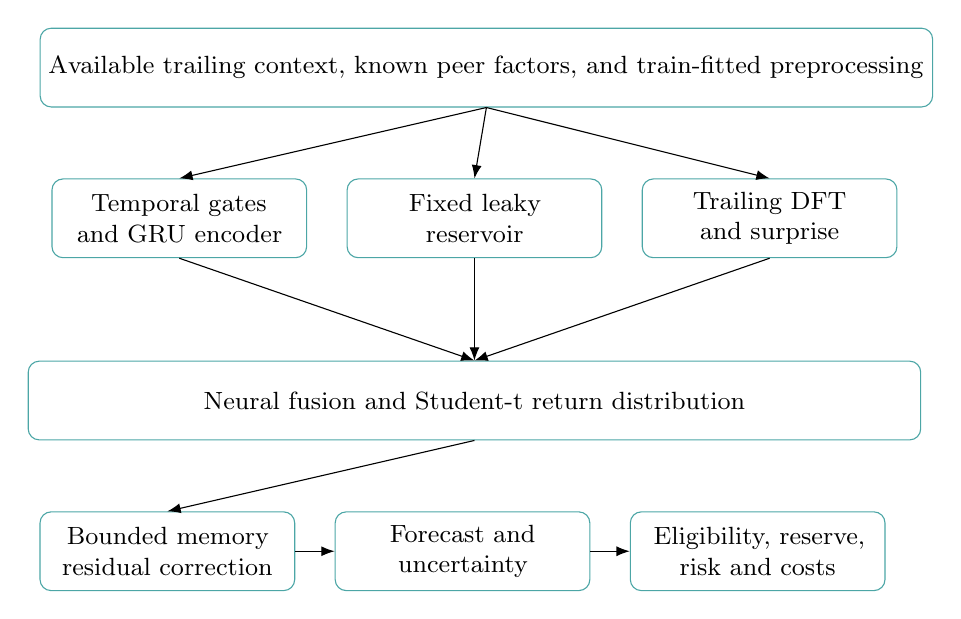
\begin{tikzpicture}[node distance=9mm and 5mm,>=Latex,
box/.style={draw=teal!70,rounded corners,align=center,font=\small,minimum height=10mm,text width=30mm},
wide/.style={box,text width=111mm}]
\node[wide] (input) {Available trailing context, known peer factors, and train-fitted preprocessing};
\node[box,below=of input,xshift=-39mm] (temporal) {Temporal gates\\and GRU encoder};
\node[box,right=of temporal] (reservoir) {Fixed leaky\\reservoir};
\node[box,right=of reservoir] (spectral) {Trailing DFT\\and surprise};
\node[wide,below=13mm of reservoir] (fusion) {Neural fusion and Student-t return distribution};
\node[box,below=of fusion,xshift=-39mm] (memory) {Bounded memory\\residual correction};
\node[box,right=of memory] (forecast) {Forecast and\\uncertainty};
\node[box,right=of forecast] (allocation) {Eligibility, reserve,\\risk and costs};
\draw[->] (input.south) -- (temporal.north);
\draw[->] (input.south) -- (reservoir.north);
\draw[->] (input.south) -- (spectral.north);
\draw[->] (temporal.south) -- (fusion.north);
\draw[->] (reservoir.south) -- (fusion.north);
\draw[->] (spectral.south) -- (fusion.north);
\draw[->] (fusion.south) -- (memory.north);
\draw[->] (memory) -- (forecast);
\draw[->] (forecast) -- (allocation);
\end{tikzpicture}
\caption{Forecast-time paths. Future contexts appear only in the training JEPA loss. Memory utility changes only after outcomes mature. Optional XGBoost residual correction is calibrated on a separate chronological interval.}
\end{figure}

\subsection{Temporal representation and relevance gates}

For each observed prefix, let $\bar x_{\tau}=\tau^{-1}\sum_{j\le\tau}\widetilde x_j$. The feature gate and the temporal gate are
\begin{equation}
g_{\tau}=2\sigma(A[\widetilde x_\tau;\bar x_\tau]+b),\qquad
a_{\tau}=2\sigma\{\operatorname{Conv}^{\mathrm{left-pad}}_3(\widetilde X)_\tau\}.
\end{equation}
A unidirectional GRU consumes $g_\tau\odot\widetilde x_\tau a_\tau$. An attention-weighted average of its hidden sequence is concatenated with its final hidden state, projected through a linear layer, GELU, dropout, and layer normalization, yielding $z_t\in\R^d$. All recurrent and convolutional dependencies lie inside the available trailing context. Attention pooling over the complete trailing window is causal at decision time even though it combines all its historical positions.

The gate-off control sets the input modulation to one and omits the learned gates. Channel relevance does not prove causal economic importance. Correlated peer features can substitute for each other, and learned gate magnitudes are diagnostic quantities rather than treatment effects.

\subsection{Contraction-bounded reservoir}

The fixed reservoir receives the scaled raw context, independently of the learned temporal gate:
\begin{equation}
r_\tau=(1-\alpha)r_{\tau-1}+\alpha\tanh(Wr_{\tau-1}+U\widetilde x_\tau+b_r),\quad r_0=0.
\end{equation}
The recurrent random matrix is rescaled so $\|W\|_2=\rho<1$, with defaults $\alpha=0.3$, $\rho=0.9$, and reservoir dimension $R=64$. Input weights have variance normalized by input dimension. Recurrent weights and biases are fixed buffers. Only the downstream fusion learns how to use $r_L$. The reservoir is reset for each context; it does not secretly accumulate an unlimited asset history.

\begin{proposition}[Forgetting of initial state]
For identical inputs and any two initial states, the reservoir obeys
\[
\|r_\tau-r'_\tau\|_2\le(1-\alpha+\alpha\rho)^\tau\|r_0-r'_0\|_2.
\]
\end{proposition}
\begin{proof}
The componentwise hyperbolic tangent is 1-Lipschitz in Euclidean norm. Apply the triangle inequality to the recurrence and $\|Wv\|_2\le\rho\|v\|_2$, then iterate. With the defaults the one-step bound is $0.97$. This is an algebraic bound, not a measured performance statistic.
\end{proof}
The result justifies bounded sensitivity to initialization under these assumptions. It does not imply financial sample efficiency, identification of hidden market states, or recoverability of information absent from the input. A strong contraction may itself erase useful long-range structure.

\subsection{Fourier descriptors and spectral surprise}

For $j=0,\ldots,L-1$, apply the Hann window $h_j=(1-\cos(2\pi j/(L-1)))/2$ to each demeaned trailing feature. The ordinary unitary real-input DFT is
\begin{equation}
C_{kd}=L^{-1/2}\sum_{j=0}^{L-1}h_j(\widetilde X_{jd}-\bar X_d)e^{-2\pi\mathrm{i}kj/L},\quad 0\le k\le\lfloor L/2\rfloor.
\end{equation}
Partition these bins into $B$ contiguous, approximately equal-sized bands. For each band $b$ and feature $d$, store the band averages of $\log(1+\operatorname{mean}_{k\in b}|C_{kd}|^2)$, real amplitude, and imaginary amplitude. More precisely, the logarithm is taken after band averaging power. Training-context means $\mu^P_{bd}$ and variances $v^P_{bd}$ of the log-power define
\begin{equation}
S_{bd}=\min\!\left(20,\frac{|P_{bd}-\mu^P_{bd}|}{\max(\sqrt{v^P_{bd}},10^{-3})}\right).
\end{equation}
The variance floor is $10^{-6}$. Learnable band weights $w_b=2\sigma(\beta_b)$ multiply the three raw descriptor channels and the surprise channel. Concatenation yields $4BD$ neural features. Mean surprise is also recorded as a candidate episode's novelty score.

This is a modified \emph{use} of a Fourier representation: a standard DFT followed by adaptive band weighting and a separate memory rule. No new transform or inversion theorem is claimed. Demeaning, a trailing window, and phase-sensitive channels do not make irregular calendar sampling equivalent to uniform physical time. The current DFT uses ordered observation indices; for markets with unequal holiday gaps, a frequency means cycles per observation. A continuous-time spectral interpretation would require a different explicit method.

\subsection{N-gram and fixed memory keys}

The most recent $p\le8$ observations of a selected scaled feature are quantized using thresholds $(-1,-0.25,0.25,1)$ into five symbols. These fixed thresholds avoid fitting a codebook on future observations. The symbol sequence is encoded as a base-5 integer and as concatenated one-hot vectors. The default is $p=3$ with the log-return feature selected by its documented index.

A memory key concatenates separately $\ell_2$-normalized blocks: the latest scaled feature vector, its trailing mean, the final fixed reservoir state, the \emph{unweighted} raw spectral descriptor, and the n-gram one-hot representation. The concatenation is normalized again and detached from gradient computation. Turning off a branch removes its corresponding key block. Key dimension is
\begin{equation}
D_k=2D+\ind_{\mathrm{reservoir}}R+\ind_{\mathrm{spectral}}3BD+\ind_{\mathrm{ngram}}5p.
\end{equation}
Frozen preprocessing, fixed reservoir buffers, and unweighted descriptors prevent learned-encoder drift from silently changing key meanings. Stored prediction residuals can still age as the predictor changes during training. Fixed keys solve one drift problem, not every nonstationarity problem.

\subsection{Retrieval, correction, and retention}

An episode stores identifier, key $k_j$, instrument, decision time $t_j$, availability $u_j$, realized log return $y_j$, residual $e_j=y_j-\mu^0_j$, n-gram code, surprise $s_j$, utility $U_j$, and credited reuse count $c_j$. A record is eligible at $t$ only when $u_j<t$ and $t_j<t$. Same-instrument retrieval is the default; exact n-gram matching is optional. Cross-instrument retrieval must be separately declared.

Among eligible records, choose the $K$ largest cosine similarities. Stable identifier order breaks ties. The retrieval weight is
\begin{equation}
\omega_j=\operatorname{softmax}_{j\in\mathcal N_t}\left(\frac{k_t^\top k_j}{T_m}-\log(2)\frac{t-u_j}{h_m}+\tanh(U_j)\right),
\end{equation}
where ages and half-life $h_m$ share units of days, with defaults $T_m=0.2$, $h_m=180$, $K=8$. All retention controls use the same similarity, age, and utility retrieval weights; only eviction changes. Memory supplies seven summaries: weighted residual mean, outcome mean, residual standard deviation, cosine similarity, $\log(1+K_t)$, utility, and a bounded age statistic. An empty store produces seven zeros.

The neural fusion concatenates $z_t$, the available reservoir state, and spectral features, then applies a linear layer, GELU, dropout, and layer normalization. Let this representation be $f_t$. The final memory gate is
\begin{equation}
\gamma_t=\ind_{K_t>0}\,q_t\,\sigma\{G([f_t;m_t])\},\qquad
\mu_t=\mu^0_t+\gamma_t\sum_{j\in\mathcal N_t}\omega_je_j,
\end{equation}
where $q_t\in[0,1]$ is a controller weight. Disabling memory yields $\gamma_t=0$. The memory gate's parameters remain present in that control, although they are inactive; actual compute differences are reported.

At a decision, the predictor schedules a pending event with its key, recorded forecasts, uncertainty, retrieved identifiers, and weights. At a later time strictly after the outcome becomes available, it computes
\begin{equation}
\Delta_t=\clip\left(\frac{(y_t-\mu^0_t)^2-(y_t-\mu_t)^2}{s_t^2+(y_t-\mu^0_t)^2+10^{-12}},-1,1\right).
\end{equation}
Retrieved episode $j$ receives $U_j\leftarrow(1-\eta_u\omega_j)U_j+\eta_u\omega_j\Delta_t$ with $\eta_u=0.1$, and its credited count increases. This is shared credit for the used correction, not a counterfactual causal attribution to an individual memory.

The new matured episode is inserted if its surprise meets the configured write threshold, which defaults to zero. Thus the default permits ordinary observations as well as anomalies. When the capacity $C=512$ is exceeded, utility retention removes the record with the smallest
\begin{equation}
Q_j=\tanh(U_j)+0.1\tanh(s_j)+0.03\log(1+c_j)-\log(2)\frac{t-u_j}{h_m}.
\end{equation}
FIFO and uniform-eviction controls preserve the declared capacity. Uniform eviction among current candidates is not uniform reservoir sampling over the entire history. Pending events have a separate explicit capacity, default $P=100{,}000$; exhaustion raises an error rather than silently discarding labels.

\subsection{Distributional prediction and stochastic interpretation}

Three return-head outputs $a_t,b_t,c_t$ define
\begin{equation}
\mu^0_t=Ha_t,\qquad s_t=\sqrt H\softplus(b_t)+s_{\min},\qquad
\nu_t=2.1+\softplus(c_t),
\end{equation}
with $s_{\min}=10^{-4}$. The predictive density is $Y_t\mid\F_t\sim t_{\nu_t}(\mu_t,s_t)$ and $\operatorname{Var}(Y_t\mid\F_t)=s_t^2\nu_t/(\nu_t-2)$. Scale is not standard deviation. The default head starts with zero return location, a 1\% step scale, and approximately five degrees of freedom. These are initialization choices, not estimated market conditions.

The $H$ and $\sqrt H$ factors give a convenient drift/scale parameterization, but they do not prove temporal aggregation consistency for dependent returns or a Student-t diffusion. The fixed-scale control trains squared error, uses a calibrated constant scale, and a high-degree Student-t approximation to a Gaussian for scoring.

\begin{proposition}[Log-Student-t arithmetic-mean limitation]
For a nondegenerate Student-t random variable $Y$ with finite degrees of freedom, $\E[e^Y]=\infty$.
\end{proposition}
\begin{proof}
Its positive-tail density decays polynomially, proportional to $y^{-(\nu+1)}$. For sufficiently large $y$, the integral of $e^y$ times any such polynomial tail diverges. Translation and positive scaling do not change this conclusion.
\end{proof}
Consequently, $\operatorname{expm1}(\mu_t)$ is a transformed location, not an expected simple return. The allocation interface refuses an undocumented substitution. One may use explicitly bounded return scenarios or a separately declared Gaussian-log-return model with finite exponential moments; either changes the distributional assumptions and must be recorded.

\section{Training and adaptive learning}

An EMA copy $\bar\theta$ of the temporal encoder defines the training-only target $z_t^+=E_{\bar\theta}(X_t^+)$. The online latent predictor $P_\theta$ is a two-layer MLP. With unit-normalized embeddings,
\begin{equation}
\mathcal L_{\mathrm{JEPA}}=\frac1{nd}\sum_t\left\|\operatorname{norm}(P_\theta(z_t))-\sg\{\operatorname{norm}(z_t^+)\}\right\|_2^2,
\end{equation}
where $d$ is latent dimension and the implemented mean-squared error averages both observations and latent coordinates. Context-embedding variance is encouraged toward at least $0.5$ standard deviation per dimension, with a $10^{-4}$ stabilizer. The covariance penalty is the sum of squared off-diagonal sample covariances divided by latent dimension. For singleton batches these terms are unidentifiable and explicitly omitted; the trainer accumulates multiple chronological groups when possible.

The supervised loss is the negative log density
\begin{align}
\ell_t={}&\log s_t+\tfrac12\log(\nu_t\pi)+\log\Gamma(\nu_t/2)-\log\Gamma((\nu_t+1)/2)\\
&+\tfrac{\nu_t+1}{2}\log\left(1+\frac{(y_t-\mu_t)^2}{\nu_ts_t^2}\right).
\end{align}
The default objective is $\overline\ell+0.1\mathcal L_{\mathrm{JEPA}}+0.01\mathcal L_{\mathrm{var}}+0.001\mathcal L_{\mathrm{cov}}$. AdamW uses learning rate $10^{-3}$, weight decay $10^{-4}$, and gradient-norm clipping at one. The target update after a neural optimizer step is $\bar\theta\leftarrow0.99\bar\theta+0.01\theta$. Target parameters receive no direct gradient, and target dropout is disabled.

Each epoch resets the episodic state and processes training decision times in order. Before a time group is forecast, previously scheduled outcomes that matured strictly earlier are released. All rows at the same decision time retrieve from the same pre-group store. Neural updates use only the training partition; validation affects the explicitly declared controller and checkpoint selection. Multiple training epochs can of course revisit the training labels, so their in-sample forecasts must not be relabeled as genuine historical out-of-sample predictions.

The learning controller has two restricted functions. First, after a prespecified number of unimproved validation scores, it reduces learning rate by a factor of $0.5$, down to $10^{-6}$, and reduces the JEPA coefficient down to a quarter of its original value. Second, matured comparisons between the base forecast and the memory-expert forecast update a bounded expert logit. The logit is clipped to $[-4,4]$ and mapped through a sigmoid. It determines $q_t$ in the memory correction. These mechanisms select the strength of predefined learning components; they do not invent architectures or optimize an arbitrary new learning algorithm.

The best validation checkpoint restores neural weights, optimizer, controller, and memory state. Validation uses the same asset-then-date balancing as the primary score; the minibatch training loss remains an observation mean. Any validation labels used to choose that checkpoint count as fitting information. Public forecasts must occur strictly after their recorded fitting-information cutoff. This rule also covers calibration labels used by the optional residual tree. A run that exhausts its budget before completing a requested validation cannot be reported as a valid selected checkpoint.

\subsection{XGBoost roles and fairness}

The standalone tree baseline consumes training-only tabular summaries of the same contexts. The optional hybrid fits XGBoost to residuals on a separate later calibration segment, using frozen neural predictions and context summaries. For residual estimate $b_t$, its correction is exactly $0.25\clip(b_t,-0.1,0.1)$, with maximum absolute cumulative log-return correction $0.025$. These fixed choices are development candidates, not optimized numerical claims.

The hybrid's tuning and calibration intervals are chronologically separated and purged within the original validation interval. It changes the use of those labels and performs an extra supervised residual fit; it does not necessarily receive more distinct observations than the basic neural candidate. It therefore belongs in an explicitly identified auxiliary comparison. The strongest information-matched claim concerns FREM ablations: classical and neural baselines use a purged internal training tail for scale calibration, whereas FREM uses the external validation interval for controller updates and checkpoint selection. Identical per-cell time caps do not by themselves equalize achieved optimization or selection opportunities. An apparent win is not evidence for memory unless these differences have been assessed. No silent substitute is used when XGBoost is unavailable: the dependency error is retained.

\section{Inference, online feedback, and mathematical guarantees}

Frozen inference loads the model, training scaler, spectral reference, fixed reservoir, memory, controller, ordered feature names, and asset mapping. It checks that decisions follow all fitting information, builds only causal context windows, retrieves eligible memory, and outputs location, scale, degrees of freedom, diagnostics, and timestamps. Unlabeled forecasts use unavailable-target markers; those markers cannot be interpreted as observed zero returns.

An explicit adaptive-inference option may release prior matured outcomes and update the episodic store and expert weight. It does not silently backpropagate through the protected evaluation set. Actual neural retraining would require a separately scheduled walk-forward protocol. A new feedback observation must identify its original decision, instrument, realized outcome, and verified availability. Conflicting corrections require an audited replay, not overwriting historical results.

\begin{proposition}[Causal forecast under a fitting cutoff]
Assume the fitted model, scaler, reference, initial memory, and controller depend only on information available by $T_0$. For every decision $t>T_0$, assume context and metadata are $\F_t$-measurable, and memory updates use only outcomes with $u<t$. Then the forecast produced at $t$ is $\F_t$-measurable.
\end{proposition}
\begin{proof}
The initialization is measurable by assumption. Induct over ordered decision-time groups. The update at a group reads only already available outcomes. Eligibility, deterministic key formation, gated neural maps, and retrieval are functions of the current context and that updated state. They therefore preserve measurability. No same-group future outcome is released. The resulting state satisfies the induction hypothesis for the next group.
\end{proof}
This guarantee is conditional on truthful provider timestamps and on not training a checkpoint using later outcomes. A false availability column defeats the assumptions even if the software's comparisons are implemented correctly.

\begin{proposition}[Bounded retained state]
With episode capacity $C$, pending capacity $P$, and fixed key dimension $D_k$, episodic and pending storage are $O((C+P)D_k)$, apart from fixed-size metadata and model parameters.
\end{proposition}
\begin{proof}
Insertion evicts whenever retained episodes exceed $C$. Scheduling rejects new events when the pending queue reaches $P$. Each record contains a fixed-length key and bounded-size retrieval metadata for fixed $K$. Thus the number and size of records have the stated bound.
\end{proof}
Stored training histories and experiment artifacts may grow with declared epochs or runs and are separate from online memory. Bounded memory does not imply bounded information loss or constant-time retrieval.

\section{Risk scenarios, markets, and constrained allocation}

The portfolio layer selects among the supplied eligible instruments. Their market, sector, asset class, currency, settlement, lot, liquidity, eligibility, and rule provenance form the allocation context. Market and sector selection occur through constrained instrument weights and their group totals. An absent market does not become investable merely because a forecast looks attractive.

\subsection{From saved marginal forecasts to portfolio inputs}

The executable forecast-to-portfolio bridge requires one common forecast time, stable ordered instrument identifiers, saved $(\mu_i,s_i,\nu_i)$, a declared base currency, and an attested common future entry and exit interval. All input provenance must be dated no later than the decision. An identical count of trading bars across different calendars is insufficient to establish a common economic horizon. The operator must verify that synchronization before the bridge is used.

Let $C$ be an explicitly supplied, dated latent Gaussian correlation matrix, or the identity only when independence is explicitly declared. For each scenario $j$,
\begin{equation}
Z_j\sim\mathcal N(0,C),\quad U_{ji}=\Phi(Z_{ji}),\quad
R_{ji}=\operatorname{expm1}\left[\clip\{\mu_i+s_iT_{\nu_i}^{-1}(U_{ji}),\,a_i,b_i\}\right],
\end{equation}
where $a_i,b_i$ are the prespecified finite log-return bounds. Numerical CDF endpoints are clamped to machine epsilon and one minus epsilon before quantile evaluation; those events are counted. The clipping operation creates probability masses at the bounds: it is winsorization, not a conditional truncated Student-t distribution. Gaussian latent correlation is neither simple-return correlation nor a Student-t copula, and its joint tail behavior is not learned by the marginal predictor.

With nonnegative declared scenario probabilities $p_j$ summing to one, the portfolio receives the finite-distribution moments
\begin{equation}
\widehat m=\sum_jp_jR_j,\qquad
\widehat\Sigma=\sum_jp_j(R_j-\widehat m)(R_j-\widehat m)^\top.
\end{equation}
There is no annualization or Bessel correction: these are exactly the moments of the retained discrete scenario distribution. Uniform Monte Carlo weights are the default; alternative weights need an explicit rationale. The decision artifact retains the scenarios, probabilities, forecast records, units, common horizon, bounds, clipping counts, dependence source, and content hashes. The bridge is one synchronous research allocation, not an executed trade or a complete portfolio backtest.

The separate raw-moment allocation interface requires an explicit simple-return, base-currency and common-horizon contract. Missing forecasts remain missing rather than becoming nonfinite array entries, allowing a documented risk-only fallback when its other required inputs are valid. An immediate cash floor is externally supplied and must be justified using the liability calculations; the bridge does not infer a ten-year funding guarantee from short-horizon forecast uncertainty.

\subsection{Scenario mathematics}

The scenario generator supports Gaussian log increments and a bounded heavy-tail alternative. Given an explicitly supplied annual drift vector $a$, annual covariance $\Sigma$, and horizon $\Delta$, the Gaussian branch starts with
\begin{equation}
Z=(a-\tfrac12\diag\Sigma)\Delta+\sqrt\Delta\,L\varepsilon,\quad LL^\top=\Sigma,\quad\varepsilon\sim\mathcal N(0,I).
\end{equation}
The heavy-tail branch multiplies the common Gaussian shock by $\sqrt{(\nu-2)/U}$ for $U\sim\chi^2_\nu$, preserving finite increment covariance when $\nu>2$. Optional shared Poisson-normal jumps represent declared systemic stress. Log increments are clipped to a recorded bound before conversion to simple returns. Even the Gaussian branch is changed by this cap; clipping frequency is therefore part of its metadata. These are hypothetical scenarios, not calibrated recession probabilities or exact samples from the neural marginal density.

Bond stress returns use an explicitly declared duration--convexity approximation, carry, and spread changes. Large yield moves, callable instruments, default, and changing cash-flow schedules can invalidate the local approximation. A real bond portfolio needs cash-flow-aware instruments and suitable issuer data. The mandate module includes liability cash-flow matching through linear programming when instrument cash flows are supplied.

\subsection{Self-financing objective and restrictions}

Let $w_i\ge0$ denote risky weights as fractions of post-cost NAV, with cash $w_c=1-\sum_iw_i$. Let $w^0$ be current risky holdings relative to pre-trade NAV $N$, and let $\alpha$ be the fraction of NAV remaining after transaction costs. Traded fractions are $d_i=\alpha w_i-w_i^0$. With per-side rates $c_i^+,c_i^-$,
\begin{equation}
\alpha+\sum_i\{c_i^+\max(d_i,0)+c_i^-\max(-d_i,0)\}=1.
\end{equation}
The implementation solves this equation before evaluating cash and traded-dollar limits. For scenario simple returns $r_s$ and cash return $r_c$, the net outcome is
\begin{equation}
R_s(w)=\alpha\{1+w^\top r_s+w_cr_c\}-1.
\end{equation}
The research objective combines predicted simple-return reward, a covariance penalty, turnover, and optional CVaR. CVaR can be represented using a threshold and upper-tail excess losses \citep{rockafellar2000}; finite weighted scenarios require fractional probability mass at a tail boundary. The package computes that tail mass explicitly.

The feasible set enforces the mandate's eligible universe, allowed markets and asset classes, security weight caps, group weight floors and caps, cash bounds, foreign-currency exposure, turnover, and dollar participation limits based on known average daily traded value. An absolute immediate-cash reserve requires $\alpha Nw_c\ge B$; that constraint alone does not certify future operating liabilities. Instrument-level foreign ownership rules and country portfolio caps are different quantities and are never interchanged. Fees, liquidity, costs, and the common forecast horizon must be explicitly supplied or declared as research assumptions.

The solver's success flag is insufficient. The proposed weights are independently checked against the same constraints. Fallbacks include keeping feasible holdings, a constrained risk-only allocation, or an eligible cash preference. Each candidate faces the same feasibility checks. If no fallback is feasible, the result is explicitly infeasible; it does not manufacture an apparently safe portfolio by violating a cash floor, mandatory sector floor, nontradable holding restriction, or turnover restriction. The instrument interface supports a dated tradable flag, not a complete settlement-accounting engine. Lot rounding requires another constraint check because continuous feasible weights need not survive rounding.

\subsection{Recession and fallback policy}

An anticipated recession is a scenario, not an established premise. The provided regime policy accepts a separately supplied recession probability, observed drawdown, volatility, data quality, forecast availability, and calibration status. Example development thresholds distinguish normal, defensive, cash-preference, and no-action states. They are configurable team policy, not legal requirements or estimated optimal boundaries. The package does not claim an autonomous, validated macroeconomic recession detector.

Data-quality or calibration failure leads to no action; unavailable forecasts can trigger a constrained risk-only fallback. A defensive setting raises risk aversion and may prefer a larger cash share while retaining hard mandate feasibility. Its value must be tested against a static policy. Transaction costs and missed recoveries can make defensive timing worse, so a fixed diversified eligible allocation remains a necessary baseline.

\section{Laura Gao case: funding before speculation}

The available source is the user's preparation document containing a copied case study \citep{laura2026}. It is stronger evidence than an earlier assistant summary, but it is not represented as an independently authenticated organizer PDF. The package preserves the document identifier, revision, case-study tab, relevant text, and access date.

\begin{table}[ht]
\centering\small
\begin{tabularx}{\linewidth}{p{.30\linewidth}X}
\toprule Case requirement & Implementation interpretation \\
\midrule Beginning 2027 & Contribution of \$300,000 \\
Beginning 2028 & Additional contribution of \$150,000 \\
Before 2033 & No other contributions or withdrawals in the stated projection \\
Beginning 2033 & Establish operating-payment reserve before first payment and any facility contribution \\
2033--2042 & Ten nominal \$50,000 payments, each at the beginning of its year \\
Facility contribution & A credible range is required in 2031; flexibility and operating obligations constrain the eventual amount \\
Outside resources & Excluded from meeting these operating obligations \\
WInS simulation results & Excluded from the long-horizon financial projection \\
\bottomrule
\end{tabularx}
\caption{Recovered case facts. Numerical risk tolerance, a confidence target, exact market allocations, and a Taiwan portfolio cap are not supplied by this case.}
\end{table}

For a specified constant net annual reserve return $r>-1$, the beginning-2033 reserve for the payments is an annuity due:
\begin{equation}
B(r)=50{,}000\sum_{k=0}^{9}(1+r)^{-k}.
\end{equation}
The first payment is undiscounted because it occurs at the reserve date. At $r=0$, the algebraic reserve is \$500,000. This is an accounting identity under the stated return assumption, not a current yield quote or a guarantee of funding. Using an end-of-year annuity would understate the needed reserve.

If annual returns for 2027--2032 are $R_y$, projected wealth immediately before beginning-2033 uses is
\begin{equation}
V_{2033}=300{,}000\prod_{y=2027}^{2032}(1+R_y)+150{,}000\prod_{y=2028}^{2032}(1+R_y).
\end{equation}
For an explicitly chosen flexibility amount $F$, a mechanical facility ceiling is $\max(0,V_{2033}-B-F)$. It becomes a responsible proposed contribution only after accounting for the distribution of $V_{2033}$, the reserve instrument cash flows, funding reliability, and the client's preferences. The 2031 update conditions on the actual then-current balance and the remaining two years of scenario returns; it does not confuse a 2026 forecast with an updated 2031 commitment.

The case does not specify a numerical funding-confidence level, flexibility reserve, approved security list, or every trading restriction. Consequently, the default Laura allocation profile remains incomplete for instrument recommendations until these inputs are documented. The cash-flow arithmetic is available independently. The official Wharton FAQ directs participants to competition materials for detailed rules and the eligible universe \citep{wharton2026}; a generic list of popular tickers cannot substitute for them.

The Taiwan example also illustrates why provenance matters. The TWSE guide describes a 10\% daily price fluctuation band for specified products, with exceptions \citep{twse2025}. That is not a universal 10\% foreign-investor portfolio or trading ceiling. A team may choose a 10\% Taiwan exposure cap as its own policy, but the configuration labels it accordingly and requires its source and effective dates.

\section{Prospective experimental design}

\subsection{Data and protected boundaries}

The first study should use a licensed, point-in-time panel with documented total-return treatment and a stable executable-observation definition. A fund or ETF panel can make distribution accounting more tractable, but it still needs historical membership and closures; present-day survivors alone are not a valid substitute. Individual equities require delistings and corporate actions. Bond or bond-fund experiments need price or total-return series rather than yields as asset returns. The same underlying asset panel is supplied to all compared methods.

The example configurations choose 1 January 2025 UTC as the protected-tail start before any dataset has been inspected in this session. This is a prospective candidate boundary, not an assertion about the available dataset. A different chosen history requires a recorded development protocol amendment before protected outcomes are viewed. Development commands filter out the protected tail before constructing windows and reporting statistics. Windows whose labels cross the protected boundary are also removed from development.

Training, validation, and development-test partitions use unique decision times. No random row split mixes adjacent windows. Purging removes samples whose label availability reaches the next partition, and an explicit embargo adds a gap. The default is five decision-time bars for a five-interval target. Purging does not eliminate every dependence; it prevents a specific label-overlap leakage route. Cross-asset dependence is handled during inference, not by pretending instruments on one date are independent.

\subsection{Models and ablations}

The primary candidate is FREM with memory, compared to its memory-off counterpart. Secondary mechanism comparisons use FIFO, uniform eviction, no spectral features, no JEPA loss, no reservoir, no n-gram descriptor, no feature gates, no adaptive controller, and fixed predictive scale. Classical and neural controls include zero expected log return, ridge, reservoir ridge, XGBoost, GRU, DLinear, and a compact patch Transformer.

Each architecture receives the same allowed context and outcomes for its declared comparison. Capacity-changing ablations report actual parameter counts and wall time. The memory-off model retains unused gate parameters, avoiding an artificial parameter-count benefit, while memory retrieval still has additional compute and storage. Equal parameter counts do not prove equal capacity. Baseline predictive scales use an inner chronological training calibration tail; refitting the point predictor afterward incurs extra work that is recorded. A strong efficiency claim requires explicit resource-matched outcomes, not only a shared nominal epoch count.

Low-data experiments take chronological suffixes containing 10\%, 25\%, 50\%, and 100\% of training dates while keeping evaluation endpoints fixed. This asks how the methods respond to fewer allowed training observations. It cannot establish reliable prediction from ``almost no data'' across arbitrary markets. Sensitivity axes include context length, reservoir size, spectral bands, memory capacity, horizon, and retention half-life. A fixed development budget bounds this search.

\subsection{Robustness and distribution shift}

Input-noise and missingness assays modify evaluation features with training-only scales and preserve targets. Missingness channels are updated where available. These assays test representation robustness, not realism of every market-data outage. OOD studies hold out declared markets, sectors, or chronological regimes. Held-out asset names must be fixed before the corresponding outcomes are inspected, and unknown assets must not accidentally reuse existing integer IDs.

Historical crisis and recovery subgroups require dates fixed independently of observed model performance. Real-time macro vintages are needed for any decision rule that would have used macroeconomic information at that time. FRED/ALFRED acquisition and availability conventions are documented separately \citep{fredapi}; date-only vintages receive a conservative delay unless actual release timestamps are available. Revised final-series recession labels are not causal input features.

Portfolio sensitivity includes spread, slippage, transaction fees, withholding and tax assumptions when applicable, FX, liquidity, participation, and cost multipliers. Predictive rows with overlapping horizons are not compounded as independent trades. The provided execution-ledger helper accepts synchronized nonoverlapping round trips and rejects asynchronous multi-market intervals. A more general multi-currency holdings simulator is a separate extension, not an invisible assumption of this release.

\section{Statistics, evidence, and stopping rules}

The primary endpoint is date-balanced Student-t negative log likelihood, a proper distributional score under its usual integrability conditions \citep{gneiting2007}. Each observation is scored using its saved, fitted location, scale, and degrees of freedom. First average complete predeclared optimization seeds per observation, repeated observations within each UTC date and instrument, instruments equally within a date, and dates equally. A seed measures optimization variability; it does not add an independent economic history.

Let $d_t=\overline\ell_t^{\mathrm{control}}-\overline\ell_t^{\mathrm{FREM}}$. Positive values favor FREM. The implementation uses a paired circular moving-date-block percentile interval and a centered-bootstrap null test. Consecutive date blocks preserve contemporaneous observations together. Block resampling is motivated by dependent observations \citep{kuensch1989}; changing regimes can still violate its assumptions. The candidate default is 20 dates, with sensitivity at 5 and 60 subject to the observed execution-and-maturity overlap lower bound, and 5,000 resamples with random seed 1901 for confirmation. A 95\% interval entirely above $0.01$ nats per observation is the prespecified practical-support criterion. This threshold is a study design choice rather than a universal scientific standard.

Exact matching of decision time, instrument, seed, realized outcome, label-availability time, and any supplied entry and exit times is required before pairing. Missing methods or seeds cause an incomplete-evidence result; inner-joining away failures is forbidden. Secondary mechanism hypotheses use the complete declared multiplicity family and Holm adjustment \citep{holm1979}. Their adjusted directional significance remains separate from the primary practical-effect criterion. Time-series dependence, limited crisis episodes, unmodeled changing opportunity sets, and few effectively independent blocks can still make inference inconclusive.

Secondary endpoints include proper distribution scores, direction probability and Brier score, interval coverage and width, MAE, date-level rank association, net wealth, drawdown, turnover, funding shortfall, actual runtime, parameter counts, memory occupancy, and resource measurements. Seed standard deviation in a descriptive figure is not a confidence interval over market histories. Sharpe and annualized quantities require a justified cadence and nonoverlapping returns; they are not produced by multiplying arbitrary horizon scores by 252.

Before confirmation, freeze code and source hashes, raw data and provenance-manifest hashes, feature schema, protected boundary, model variants, hyperparameters, seed family, primary endpoint, practical threshold, exclusions, stopping rules, and environment. Verification rejects changed identities. Each run archives the exact analysis protocol, and confirmatory analyses verify its frozen hash and settings. A consumption receipt prevents accidental reuse of the same confirmatory freeze, including after interruption. This is an operational research guard, not protection against an owner deliberately altering their files. Protected outcomes cannot be used to revise that version's central hypothesis. A new scientific change becomes a successor version with the original result retained.

The valid terminal categories are supported, mixed, negative, and inconclusive. Invalid is an evidence-quality state requiring an explicit defect description and corrected protocol. A valid negative result is accepted; repeated evaluation solely to obtain a favorable seed is prohibited. The current state remains \textbf{not evaluated}, which is different from an empirical inconclusive result.

\section{Computational complexity and engineering limits}

For one context, a dense reservoir costs $O(L(R^2+RD))$, the spectral transform $O(DL\log L)$, and a GRU approximately $O(L(d^2+dD))$. Spectral pooling and fusion add costs proportional to the actual descriptor dimensions. Exact memory retrieval costs $O(CD_k+C\log C)$ with the current full candidate ordering, plus $O(K)$ summary work. Pending-queue scans are $O(P)$ per advance in the straightforward implementation. These terms can dominate before neural compute on small models.

No claim of improved tokens per second, training speed, or energy use is made. A dense fixed recurrence reduces trainable parameters in one branch but still performs recurrent matrix multiplication. A FIFO comparison and a no-memory comparison help reveal whether predictive gains justify lookup overhead. Optimizations such as approximate search, heap-based maturity queues, and batched fixed-key caching may be useful successors, but they require equivalence or changed-method evaluation before replacing the frozen implementation.

The default device is CPU, appropriate for a first bounded compatibility run on a modest machine. Runtime performance has not been measured. PyTorch's complex FFT path is not assumed portable to every accelerator backend; the trainer explicitly rejects unsupported spectral MPS use rather than silently changing its computation. Checkpoints preserve model buffers, EMA targets, optimizer, scaler, memory, controller, schemas, and fitting cutoffs. Baseline persistence follows the relevant estimator format, and pickle-derived files must be treated as trusted local artifacts only.

Experiment directories are unique, retain partial outputs, record failures and interruptions, and include environment and source identities. Process peak RSS is explicitly a process-lifetime high-water mark rather than isolated per-model memory. Cooperative wall-time limits are checked during training and between matrix cells. A single native tree fit is not forcibly interrupted by that API; a scheduler-level hard timeout is needed when hard resource containment matters.

\section{Adversarial audit and required evidence}

\begin{longtable}{>{\raggedright\arraybackslash}p{.23\linewidth}>{\raggedright\arraybackslash}p{.31\linewidth}>{\raggedright\arraybackslash}p{.37\linewidth}}
\toprule Objection & Mechanism or cause & Repair and required evidence \\
\midrule\endhead
The combination is not novel & All major ingredient families predate this study & Restrict novelty to the retention hypothesis; compare direct neighbors and do not claim a new Fourier transform \\
Memory stores noise & Rare events need not recur or predict returns & Compare utility, FIFO, uniform, and no memory; inspect delayed utility and retrievals \\
Memory exploits hindsight & Future labels or revised data enter too early & Timestamp gates, vintage provenance, same-time grouping, maturity tests, protected tail \\
JEPA collapses or hurts & Predictable latent features may become trivial or irrelevant & Latent variance/covariance diagnostics, anti-collapse losses, JEPA-off control \\
Low-data claims are overstated & Priors cannot recover absent signal & Fixed low-data curves, zero/ridge controls, uncertainty, accepted null outcomes \\
Spectral artifacts dominate & Windowing, irregular sampling, changing price scale & Return-based features, trailing DFT, explicit observation-time meaning, window/horizon sensitivity \\
Residual memory becomes stale & Neural predictor and market drift & Fixed keys, age decay, utility credit, residual-drift analysis; no guarantee of stationarity \\
Learning controller just tunes more & Extra validation reuse favors one method & Fixed policy and budget, controller-off comparison, report all tuning information \\
Trees explain the win & Additional model capacity or calibration labels & Standalone XGBoost, separate hybrid comparison, matched-information interpretation \\
Uncertainty is misused & Scale confused with SD or log mean with price mean & Save degrees of freedom, exact scoring, calibration, explicit bounded simple-return scenarios \\
Funding reserve is optimistic & Constant-rate assumptions hide sequence risk & Annuity-due timing, scenario reserve paths, cash-flow matching, no outside-funding assumption \\
Cross-market backtest is unrealizable & Different close times, holidays, FX, and fills & UTC availability, synchronized ledger restriction, explicit portfolio-engine extension \\
Defaults disappear & Log returns cannot represent zero recovery & Fail and record the defect; add a default-mass model in a successor rather than exclude failed issuers \\
Good results are selection artifacts & Many variants and repeated holdouts & Frozen protocol, complete seed family, date blocks, multiplicity and failure retention \\
Fallback violates rules & Cash or reduced turnover is assumed always feasible & Recheck all hard constraints for every fallback and after lot rounding \\
\bottomrule
\end{longtable}

\section{Current evidence, release gates, and handoff}

This version contains source implementations, configuration files, written tests, source provenance, mathematical documentation, and explicit experiment commands. The original research pipeline is preserved in the package. The user's preparation document also reports negative synthetic APEN-memory and larger graph-memory comparisons. Their exact excerpts and verification status are retained; underlying runs were not independently re-audited in this session, and this new implementation does not demonstrate that those failures are solved. Static authoring review is not empirical execution, and it cannot establish that every dependency combination or data-provider export works at runtime. Detailed static findings and remaining execution gates are in the release verification record.

The next executable sequence is: install and record an environment; run the provided tests; validate a bounded pre-protected dataset; perform the small development dry run; review leakage, scale, memory, and baseline behavior; run only the selected bounded development matrix; freeze the final confirmatory protocol; and then evaluate the untouched tail once. A runtime defect found at any gate must be fixed and recorded before advancing. Model weights and market data are absent because they were not generated or downloaded.

The paper's empirical sections must later be populated from saved predictions, manifests, and paired analyses. No placeholder numerical tables masquerade as results. Figure and report generators refuse missing or incomplete evidence. A submission-ready manuscript additionally requires actual experiments, a final related-work audit, author approval, venue-specific formatting, verified data rights, and a complete claim-to-artifact check.

\section{Conclusion}

FREM defines an implementable financial forecasting hypothesis: stable trailing descriptors can retrieve a bounded set of episodes whose retention responds to matured predictive utility. The model incorporates temporal latent prediction, fixed recurrent features, spectral weighting, motif keys, restricted adaptive learning, and explicit uncertainty. The allocation system treats legal eligibility, costs, and liability funding as separate constraints on how forecasts may be used. The mathematical guarantees concern causal access, bounded memory, and reservoir forgetting under stated assumptions; they do not prove returns, low-data success, or efficiency. Whether the proposed memory improves useful prediction remains the task of the frozen experiments.

\appendix
\section{Implementation map}
\begin{longtable}{>{\raggedright\arraybackslash}p{.32\linewidth}>{\raggedright\arraybackslash}p{.59\linewidth}}
\toprule Module & Responsibility \\
\midrule\endhead
\texttt{data.py} & Schema, provenance validation, causal features, windows, unlabeled inference, train-only scaling \\
\texttt{data\_sources.py} & Explicit macro-vintage acquisition and provenance-preserving loading \\
\texttt{splits.py} & Purged chronological and walk-forward partitions \\
\texttt{model.py} & Temporal encoder, reservoir, spectral operator, return density, JEPA loss \\
\texttt{memory.py} & Timestamped episode retrieval, pending feedback, utility, eviction \\
\texttt{controller.py} & Declared learning schedules and matured expert weighting \\
\texttt{training.py} & Chronological fitting, EMA, validation, inference, checkpoints, residual tree \\
\texttt{baselines.py} & Classical, tree, recurrent, linear-decomposition, patch sequence controls \\
\texttt{metrics.py}, \texttt{evaluation.py} & Distributional scores and realizable nonoverlapping return accounting \\
\texttt{statistics.py} & Complete-seed aggregation, date-block inference, multiplicity \\
\texttt{mandate.py} & Rules, provenance, eligibility, cash flows, reserves, facility analysis \\
\texttt{risk.py}, \texttt{portfolio.py} & Explicit scenarios, covariance, regime policy, constrained allocations and fallbacks \\
\texttt{decision.py} & Dated forecast/horizon contracts and bounded scenario conversion into one research allocation \\
\texttt{experiments.py}, \texttt{robustness.py} & Bounded matrices, ablations, data-size and perturbation studies \\
\texttt{governance.py}, \texttt{artifacts.py} & Freezes, identities, unique runs, failure records, decision journal \\
\texttt{reporting.py}, \texttt{cli.py} & Evidence-derived outputs and explicit user commands \\
\bottomrule
\end{longtable}

\section{Research-stage accounting}
The idea and mathematical implementation contract are specified. Source code for the model and methodology is supplied. Runtime calibration, dry-run readiness, measured efficiency, scientific development, confirmatory freeze, protected evaluation, evidence locking, independent reproduction, and final empirical release remain uncompleted by design. Their future outputs are not implied by this manuscript's existence. The canonical state must be updated after each actual execution, retaining failures and superseded hypotheses.

\bibliographystyle{plainnat}
\bibliography{references}
\end{document}
